\chapter{\textbf{MapReduce}}

MapReduce é sistema de programação de alto nível que permite que muitos processos de um 
banco de dados (BD) possam ser escrito de forma simples, de acordo com Molina \cite{Molina}.
Esses processos dos bancos de dados visam processar um grande quantidade de dados, que
são divididos e designados a um conjunto de máquinas, denominado
cluster de computadores. Tem por objetivo melhorar o desempenho na performance
obtida pelo paralelismo, omitindo toda a complexidade de modo que o usuário
foque no problema principal, que é o processamento dos dados.

O modelo MapReduce é composto por duas fases, a de mapeamento dos dados e
redução. Para execução dessas fases o framework designa uma das
máquinas do cluster como master; essa máquina então define um conjunto de
máquinas para desempenhar a função de mapeamento e um outro conjunto para
executar a tarefa de redução. Na primeira fase a máquina master tem a função de
dividir os dados de entrada em várias partes menores e então designar cada parte
a uma máquina que estará desempenhando a atividade de mapeamento. Após o término
dessa fase inicia-se a fase de redução. Nessa segunda fase a máquina master
notificará as máquinas que desempenham a atividade de redução sobre a
localização dos dados produzidos pela fase anterior, para que os dados sejam
condensados em informações úteis para que possam ser interpretados e utilizados
para o fim necessário. Podemos ver a execução na figura \ref{MapReduce}.

\begin{figure}[ht]
  \centering
  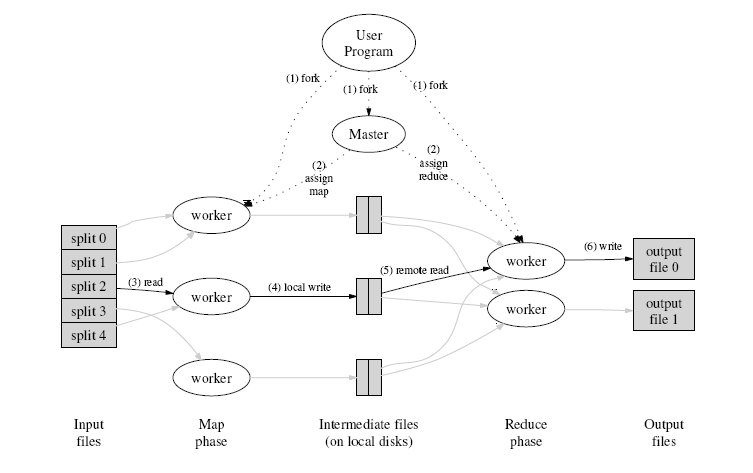
\includegraphics[width=400px,height=400px]{img/mapreduce.png}
  \caption{Visão geral da execução do framework MapReduce\newline
  Fonte: MapReduce: Simplified Data Processing on Large Clusters (2004, p. 3)}
  \label{MapReduce}
\end{figure}

Cada uma dessas fases, a de mapeamento e redução, implementa uma função, Map e 
Reduce respectivamente, ambas funções são implementadas pelo usuário.

A função Map recebe como entrada um par chave-valor. Com o par serão realizadas
as operações definidas (operações de Map e Reduce), e será produzido como saída
uma lista de pares chave-valor intermediárias. Com a conclusão dessa fase o
framework agrupará todos os valores associados a mesma chave, partindo para a
próxima fase, que utiliza a função Reduce.

A função Reduce recebe como entrada o par chave-lista de valores associada a
chave. O objetivo dessa função é realizar tarefas para agrupar ainda mais os
valores associados a mesma chave, gerando, normalmente, uma única saída.

Algumas variações do modelo são possíveis para que ele se adapte melhor as
características dos dados analisados e operações realizadas pelas funções Map e
Reduce, visando uma melhor performance na utilização do modelo. 

\section{\textbf{Hadoop}}

Hadoop \cite{hadoop} é um framework que permite o processamento de dados em
larga escala em clusters de computadores. Oferece um mecanismo de distribuição
dos dados em um Sistema de Arquivo Distribuído (Hadoop Distributed File System - HDFS)
ver \cite{hdfs}. Também oferece uma interface para implementar as funções de Map e 
Reduce o que facilita a programação.

As premissas do MapReduce consiste na simplificação do armazenamento, comparada
as estruturas de armazenamento do SGBD, o armazenamento utilizado deve ser
simples e normalmente armazenar uma chave e um valor para os dados.

O Hadoop pode ser instalado em três modos: Standalone, Pseudo-Distributed e
Fully-Distributed. A primeira é útil para testar a aplicação e depurar o código,
e roda como um único processo Java. O modo Pseudo-Distributed, assim como no
Standalone, é executado em apenas uma máquina, porém cada daemon do Hadoop roda
em um processo distinto. Já o modo Fully-Distributed é utilizado em sistemas de
produção, realmente distribuídos.	

Preocupações com falhas de hosts no meio de processamento de tarefas são
desconsideradas. Todos os problemas de distribuição ficam a cargo do framework.

\section{\textbf{Hive}}
Hive \cite{hive} é uma infra-estrutura de data warehouse construída em cima do
Hadoop. 

Ele suporta convenientemente a análise de grandes conjuntos de dados armazenados
em sistemas de arquivos compatíveis com o Hadoop,  como exemplo o sistema de
arquivos  da Amazon S3 \cite{amazon}. Ele fornece uma linguagem SQL-like chamado HiveQL
mantendo total apoio para o MapReduce. Para acelerar consultas, fornece índices
como o índice de bitmap. Um exemplo de arquitetura com o Hive é do facebook
conforme a figura \ref{hive}.

\begin{figure}[ht]
  \centering
  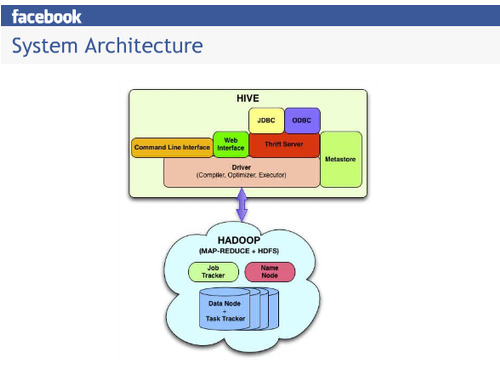
\includegraphics[width=300px,height=200px]{img/hive2.png}
  \caption{Facebook Data Infrastructure\newline
  Fonte: http://nosql.mypopescu.com/post/681603154/presentation-hive-a-petabyte-scale-data-warehouse}
  \label{hive}
\end{figure}
 
Atualmente, existem três formatos de arquivos suportados no Hive, que são
textfile, SEQUENCEFILE e RCFILE.


